\documentclass[UTF8]{ctexbeamer}
% for old TeX systems, please use the following alternate
% \documentclass[notheorems]{beamer}
% \usepackage[UTF8]{ctex}
\usepackage{latexsym}
\usepackage{amsmath,amssymb}
\usepackage{color,xcolor}
\usepackage{graphicx}
\usepackage{algorithm}
\usepackage{amsthm}
\usepackage{unicode-math}

\usetheme{AnnArbor}
\usefonttheme[onlymath]{serif}
\usecolortheme{spruce}


\title[论文复现报告]{Vision Transformers in 2022:
An Update On Tiny-imagenet}
\author[董宇坤]{董宇坤 PB21000237}
\institute[ustc]{dyk2021@mail.ustc.edu.cn}
\date[\today]{\today}
\begin{document}


\begin{frame}
    \titlepage
\end{frame}

\begin{frame}{论文概要信息}
  \begin{itemize}
    \item 作者:Ethan M. Huynh,University of California, San Diego
    \item 发表时间:21 May 2022
    \item 数据集:tiny-imagenet
    \item 论文长度:共6页
  \end{itemize}
\end{frame}

\begin{frame}{0.摘要(Abstract)}
  \kaishu {近期的图像转换器技术有了重大进步,并在一定程度上缩小了与传统
  CNN架构之间的差距。标准的处理流程是先在像ImageNet-21k这样的大型数据
  集上进行训练,然后再在ImageNet-1k上进行微调。微调之后,研究者们通常
  会考虑在像CIFAR-10/100这样的小型数据集上进行\textcolor{blue}{迁移学习}的性能,
  但往往会忽略Tiny ImageNet数据集。\textcolor{blue}{本文为视觉转换器在Tiny ImageNet上的性能提供
  了更新}。包括了视觉转换器(Vision Transformer,ViT),数据高效图像转
  换器(Data Effificient Image Transformer,DeiT),图像转换器中的类
  别注意力(Class Attention in Image Transformer,CaiT)以及Swin转
  换器(Swin Transformers)。此外,\textcolor{blue}{Swin转换器以91.35\%的验证准确率超
  越了当前的最优结果}。}
  \begin{block}{remark}
    迁移学习意味着训练该模型需要调用预训练模型;摘要提到了四种转换器(transformer),
    训练这四种转换器并且比较他们的性能是此次论文复现的主要目标。
  \end{block}
\end{frame}

\begin{frame}{1.简介(Introduction)}
  \kaishu ViT论文(Dosovitskiy等人,2020年)展示了可以将转换器应用于图像分类
  任务。然而,ViT是在JFT-300M数据集(Sun等人,2017年)上预训练的,这是Google
  的内部数据集,包含了3亿张图片。因此,训练效率和数据可用性的问题就显而易见了。
  \textcolor{blue}{DeiT(Touvron等人,2020年)对此做出了回应,表明了缓解 Transformer 数据匮乏性
  质的一种方法是通过严格的培训计划和知识提炼}。因此,可以使用ImageNet-21k(Ridnik等人,
  2021年)来训练视觉转换器,并在ImageNet-1k(Russakovsky等人,2014年)上进一
  步微调。像CaiT(Touvron等人,2021年)和Swin(Liu等人,2021b年)等后续的图像
  转换器,都紧密遵循了DeiT所制定的蓝图。

  除了ImageNet-1k,这些研究还在CIFAR-10和CIFAR-100(Krizhevsky,2009年)上进
  行迁移学习测试。\textcolor{blue}{然而,每一篇论文都没有包含Tiny ImageNet}(Le \& Yang,2015年)。
  Tiny ImageNet是ImageNet-1k的一个子集,包含了100,000张图片和200个类别,最初
  在斯坦福大学的一个计算机视觉课程中被介绍出来。自从它的诞生以来,很少有论文在
  他们的基准测试中使用这个数据集。
\end{frame}

\begin{frame}{1.简介(续)}
  \kaishu   
  也就是说,Lee等人(2021年)做过一项研究,他们提出了修改视觉转换器的方法,以提
  高在Tiny ImageNet上从零开始训练的准确性。但实际上,当涉及到准确性时,迁移学习
  是一种更常见且更强大的技术。因此,没有现代研究对Tiny ImageNet上的视觉转换器进
  行评估。\textcolor{blue}{本文将填补这个空白,并报告使用与DeiT类似的训练制度的ViT,DeiT,CaiT,
  和Swin转换器的准确性}。
\end{frame}

\begin{frame}{2.实验设置(Experimental Setting)}
  \begin{itemize}
    \item 所有的视觉转换器都来自于timm库(Wightman,2019)
    \item 使用Nvidia RTX 3070(8GB内存)和8核CPU训练每个模型
    \item 每个epoch训练的时间在10到60分钟之间来选择
  \end{itemize}
  \begin{table}[h]
    \centering
    \begin{tabular}{|l|l|l|l|}
    \hline
    Model & ImageNet-1k & CIFAR-100 & CIFAR-10 \\
    \hline
    ViT-L/16 & 87.08 & 94.04 & 99.38 \\
    DeiT-B/16-D & 85.43 & 91.40 & 99.20 \\
    CaiT-M/36 & 86.05 & 93.10 & 99.40 \\
    Swin-L/4 & 87.15 & - & - \\
    \hline
    \end{tabular}
    \caption{Results of ViT, DeiT, CaiT, and Swin on ImageNet-1k, 
    CIFAR-100, and CIFAR-10}
    \end{table}
\end{frame}

\begin{frame}{2.1数据增强(Data Augmentation)}
  作者参考了DeiT的的相关工作,使用了数据增强技术,要点和参考的来源如下:
  \begin{itemize}
    \item 分别以0.8和1.0的概率使用Mixup(Zhang等人,2017)和Cutmix(Yun et al.
    ,2019)
    \item 以概率0.25使用Random Erasing(Zhong等人.,2017)
    \item (Touvron,2020)在训练和测试中使用尺寸调整为 384x384 分辨率的完整图像并
    加以使用双三次插值算法(bicubic interpolation)
  \end{itemize}
\end{frame}

\begin{frame}{2.2正则化和优化器(Regularization and Optimizer)}
  \begin{block}{正则化}
    使用标签平滑(Label Smoothing)正则化方法,参数$\epsilon = 0.1$,随机深度取0.1。

    训练每个模型采用batch size=128,epochs=30。由于图像分辨率为384x384,8GB的
    显存不足以将模型和批量加载到GPU内存中。因此,需要使用梯度累加
    (gradient accumulation)来训练batch size为128的模型。
  \end{block}
  \begin{block}{优化器}
    选择的优化器是AdamW,初始学习率为$10^{-3}$,余弦衰减和权重衰减为0.05。
  \end{block}
\end{frame}

\begin{frame}{3.文章的结果(Results)}
  \begin{table}[h]
    \centering
    \begin{tabular}{|l|l|l|l|}
    \hline
    Model & Tiny ImageNet & \#params & FLOPs \\
    \hline
    ViT-L/16 & 86.43 & 304M & 190.7B \\
    CaiT-S/36 & 86.74 & 68M & 48.0B \\
    DeiT-B/16-D & 87.29 & 87M & 55.5B \\
    Swin-L/4 & \textbf{91.35} & 196M & 103.9B \\
    \hline
    \end{tabular}
    \caption{Analysis of ViT, DeiT, CaiT, and Swin accuracy and training
     efficiency on Tiny ImageNet.The highest validation accuracy during training is reported.}
    \end{table}
    \begin{itemize}
      \item Swin 转换器以 91.35\% 的验证准确率超越了当前的最优结果。将
      一个窗口应用于多头自注意力(MSA)和一个平移窗口应用于 MSA 已经被证明
      是有效的。
      \item DeiT 达到了可观的 87.29\% 的准确度,同时以大幅度的优势训练得
      最快。数据增强的力量显而易见,因为它比 ViT-L 表现得更好,并且训练速度
      以很大的优势领先。
      \item CaiT-M/36 模型可能会超过 DeiT 模型。
      尽管参数个数和 FLOPs 的数量较少,CaiT 的训练时间却是最长的。
    \end{itemize}
\end{frame}

\begin{frame}{3(\ast).复现结果}
  在训练精度上,我的训练结果与论文的结果高度相近,可以说是高度复现,论文的真实性与
  可再现性得到了基本的证实。
  \begin{table}[h!]
    \centering
    \begin{tabular}{|c|c|c|c|}
    \hline
    model & (paper)acc@1 & (my)acc@1 & (my)acc@5 \\
    \hline
    ViT-L & 86.43 & \textbf{86.52} & 95.82 \\
    CaiT-S36 & 86.74 & 86.66 & 96.61 \\
    DeiT-B distilled & 87.29 & \textcolor{gray}{82.52} & 94.16 \\
    Swin-L & 91.35 & 91.20 & 98.01 \\
    \hline
    \end{tabular}
    \caption{复现结果与论文对比}
    \end{table}
\end{frame}

\begin{frame}{3(\ast).复现结果}
  DeiT模型的准确率不够理想,怀疑是训练进程多次中断,断断续续调出来而导致的。
  也有可能是,消融实验得到的一些最优参数和最优方法的选择不一定适用于所有的模型。
  注意到此时模型DeiT使用的batch size为64,因此我又换了batch size重新实验,
  得到以下结果:
  \begin{table}[]
    \centering
    \begin{tabular}{|c|c|c|c|}
    \hline
    DeiT-B training batch size & (paper)acc@1 & (my)acc@1 & (my)acc@5 \\ \hline
    32 & & & \\ \hline
    64 & 87.29 & & \\ \hline
    128 & & & \\ \hline
    \end{tabular}
    \caption{复现结果与论文对比(续)}
    \end{table}    
\end{frame}

\begin{frame}{3(\ast).复现结果}
  \begin{table}[h!]
    \centering
    \begin{tabular}{|c|c|c|c|}
    \hline
    Model & (my)acc@1 & storage space & time per epoch \\
    \hline
    ViT-L/16 & 86.52 & 1.13GB & 22:56 \\
    CaiT-S/36 & 86.66 & 781MB & 23:10 \\
    DeiT-B/16-D & 82.52 & 330MB & 9:20 \\
    Swin-L/4 & 91.35 & 761MB & 20:30 \\
    \hline
    \end{tabular}
    \caption{模型性能对比}
  \end{table}
    
\end{frame}

\begin{frame}{3.1参数个数和FLOPs的影响并非均等}
  CaiT模型显示,参数数量和FLOPs并不能准确反映模型的效率。尽管CaiT-S/36有最少
  的参数数量和FLOPs,但它的工作量最低,训练速度最慢。相反,层次的数量
  和工作量之间存在一种趋势。嵌入的大小是另一个需要考虑的因素,但考虑到CaiT的嵌
  入尺寸较小,层次的数量似乎是主要的决定因素。
  \begin{table}[h]
    \centering
    \begin{tabular}{|c|c|c|c|c|c|}
    \hline
    Model & \#layers & Embedding Size & Throughput (images/sec)\\
    \hline
    ViT-L/16 & 24 & 1024  & 31.5 \\
    \hline
    CaiT-S/36 & 36 & 368  & 24.0 \\
    \hline
    DeiT-B/16-D & 12 & 768  & 83.1 \\
    \hline
    Swin-L/4 & 18 & 192  & 36.0 \\
    \hline
    \end{tabular}
    \caption{Comparison of various model size metrics with throughput.}
    \end{table}
\end{frame}

\begin{frame}{4.1.训练过程讲解之超参数}
  \begin{itemize}
    \item 优化器方面:对于AdamW,作者尝试了学习率和权重衰减的组合,范围分别为
    $[3.10^{-3}, 10^{-3}, 7.10^{-4}, 5.10^{-4}]$和$[0.2, 0.05, 0.01]$。实验表明$10^{-3}$
    的学习率和0.05的权重衰减效果最好。
    \item 作者也考虑了扰动优化器,如SAM(Foret等人,2020),ASAM(Kwon等人,2021)和
    PUGD(Tseng等人,2021)。初步测试显示,SAM,ASAM和PUGD将一个epoch的训练时间增
    加了85\%,而前五个epoch的准确率仅在60-70\%左右。相比之下,AdamW在第一个epoch后
    的准确率为89\%。因此,作者决定不使用这些优化器进行训练。
  \end{itemize}
\end{frame}

\begin{frame}{4.1.训练过程讲解之超参数}
  \begin{itemize}
    \item 此外,作者还测试了SGD,学习率为$10^{-2}$,权重衰减为$10^{-5}$,动量为
    $0.9$,包括有或没有nesterov动量两种情况。
  \end{itemize}
  \begin{center}
    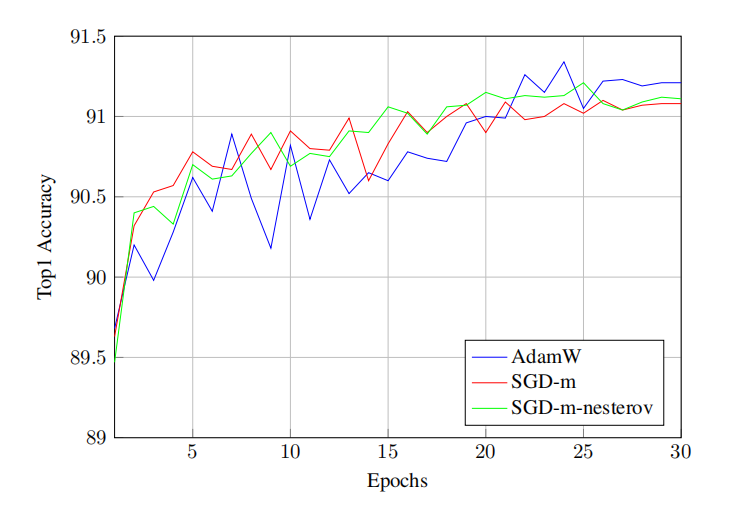
\includegraphics[width=0.8\textwidth]{1.png}
  \end{center}
\end{frame}

\begin{frame}{4.1.训练过程讲解之超参数(续)}
  上图显示,SGD比AdamW收敛更快,这可能是因为作者为SGD使用了更高的学习率。另一方面,
  AdamW比SGD变化更大,这可能是由于AdamW的自适应性质。无论如何,就准确率而言,
  SGD均不如AdamW,但是nesterov动量的表现优于普通动量(91.21\%对比91.1\%)。
\end{frame}

\begin{frame}{4.2.消融实验(Ablation Study)}
  本节描述了移除各种数据增强和正则化技术,以及尝试不同技术对于在Tiny ImageNet
  上训练Swin的影响,以确定最优的训练设置。

  \begin{itemize}
    \item 默认训练设置:自动增强(Cubuk等人,2018)、图像裁剪和模型EMA
    \item 尝试了两种裁剪方式,随机重设裁剪(RRC)和简单随机裁剪(SRC)
    (Touvron等人,2022)
    \item 模型EMA表明,在某些情况下,它可以提高精度,在某些情况下,
    它可能会降低精度。Liu等人(2021b)报告说模型EMA没有帮助,但是仍值得
    在数据集级别上进行尝试。
  \end{itemize}
\end{frame}

\begin{frame}{4.2.消融实验(续)}
  \begin{table}[h]
    \centering
    \caption{Comparison of the effects of various data augmentation and regularization techniques. RA stands for Rand-Augment.}
    \begin{tabular}{|l|r|}
    \hline
    \textbf{Change} & \textbf{Accuracy} \\
    \hline
    Default & 91.34 \\
    Remove RandAugment & \textbf{91.35} \\
    Remove Rand-Erasing & 91.28 \\
    Add Simple Random Crop & 91.26 \\
    Remove Stochastic Depth & 91.25 \\
    Remove Label Smoothing & 91.25 \\
    Replace RA with AutoAugment & 91.25 \\
    Remove Mixup & 91.11 \\
    Add Random Resized Crop & 91.06 \\
    Remove CutMix & 91.04 \\
    Add Model EMA & 90.83 \\
    \hline
    \end{tabular}
    \end{table}    
\end{frame}

\begin{frame}{4.3.消融实验的结果(Ablation Results)}
  作者详细讨论了在Swin模型上使用不同的数据增强和正则化技术的影响:
  \begin{itemize}
    \item RandAugment是唯一降低训练精度的技术,作者选择移除它
    \item 尽管AutoAugment和Model EMA在实验中表现出精度下降,但作
    者认为对AutoAugment进行一些参数调整可能会有所帮助
    \item 其他的裁剪方法在实验环境中没有表现出有效性,可能是因为在
    预训练和微调阶段已经进行了裁剪
  \end{itemize}
\end{frame}

\begin{frame}{4.3.消融实验的结果(续)}
  作者给出了最优的训练设置配置如下:
  \begin{itemize}
    \item AdamW,学习率为$10^{-3}$,权重衰减为0.05
    \item 30 epochs, 余弦衰减, and batch size=128
    \item Mixup
    \item CutMix
    \item 随机深度为0.1
    \item 标签平滑为0.1
  \end{itemize}
\end{frame}

\begin{frame}{5.结论(Conclusion)}
  \kaishu
  论文表明,\textcolor{blue}{视觉变换器(vision transformers)在Tiny ImageNet上的迁移性能很好},这是合理的,因为它
  是ImageNet-1k的一个子集。\textcolor{blue}{两个突出的架构是DeiT和Swin。DeiT在训练最快的同
  时,报告了一项相当可观的准确性,而Swin达到了最先进的准确性,比以前提高了
  0.33\%}。未来可以在更多的视觉变换器上进行工作。SwinV2(Liu等人,2021a)改
  进了Swin,并使用自我监督学习技术和后规范化等手段扩大了Swin。另一个是MiniViT
  (Zhang等人,2022),它使用了权重共享和权重蒸馏的组合,极大地减少了参数数量,
  并提高了视觉变换器的准确性。
\end{frame}

\begin{frame}
  \centering
  \Huge Thank You!
\end{frame}

\end{document}
